\subsection{Page conditioning and line segmentation}
\label{sec:segmentation}

The first block of the classification chain (functional units FU~2.1 and FU~2.2 of the proposal) turns a photograph of a handwritten page into clean, deskewed, white-background line images for the text recogniser (Section~\ref{sec:textrec}) and the writer classifier (Section~\ref{sec:writerid}).
The deployed implementation is the module \texttt{Software/CleanPipeline/SegmentLean.py}, and its entry point is the single function \texttt{SegmentLines(path)}, which takes the path of one photograph and returns a list of line records, a debug overlay image and a dictionary of page statistics.
That function is the segmenter of the whole system: the web server calls it (\texttt{Server.py}, \texttt{SL.SegmentLines}), and so do the style-profile builder (\texttt{BuildStyleProfile.py}) and the writer-classifier training program (\texttt{TrainAuthor.py}), so the pages used for training are cut by exactly the same code that cuts a page at inference time.
The module is deliberately small: eleven functions in about 570 lines, of which seven are reusable array primitives and one is the pipeline itself.

Every decision rule in the module --- the threshold, the skew objective, the run-length tests, the profile peak picking, the dynamic program, the ownership rules and the crop rendering --- is the student's own code written in plain array arithmetic over NumPy arrays.
Pillow is used for four mechanical operations only: reading the image file and converting it to grey scale, resampling (the $2{:}1$ reduction, the rotation, and the enlargement of the background estimate and of the line masks back to full resolution), and drawing the coloured cut lines on the debug overlay.
\mustdo{declaration~6 of the preamble states that Pillow was used only for reading and writing image files. \texttt{SegmentLean.py} also calls \texttt{Image.resize} and \texttt{Image.rotate}, which are resampling routines, inside the signal path. Either widen declaration~6 to name resampling explicitly or replace those two calls with the project's own bilinear sampler (Equation~\ref{eq:seg-resize} already gives the rule).}

\subsubsection{Motivation and design goals}

Requirement R2 demands that the content and the writer are decoded from a photographed page and requirement R4 allows 2\,s for capture and conditioning; both depend on this block, because a badly cropped line cannot be repaired by the networks that follow.
A photograph differs from a flat-bed scan by seven nuisances the block has to remove: uneven illumination (a lamp gradient or a shadow), the surroundings of the sheet (desk, hand, neighbouring page), skew, printed structure (ruled and margin lines touching the handwriting), faint marks (bleed-through, pale print, lightly pressed strokes), page-boundary artefacts (edge slivers, corner shadows, fold creases) and touching lines (descenders meeting ascenders).
The block shall therefore work for any camera resolution and handwriting size without manual tuning (goal~a), never delete handwriting to remove a nuisance (b), be cheap enough in operation count that a single-board computer is not excluded on algorithmic grounds (c), and keep the number of tunable constants small enough that each one can be justified individually (d).

Goal~(a) is met by \emph{scale invariance against a measured quantity}.
The module does \emph{not} normalise the photograph to a fixed pixel size.
It works on the captured image reduced by exactly $2{:}1$, measures the \emph{line pitch} $P$ --- the vertical spacing between consecutive text lines, in pixels of that half-resolution image --- from the page itself, and expresses almost every subsequent threshold as a multiple of $P$ (for example a piece of ink is ``thin'' if it is narrower than $0.5P$, and a candidate ink dot must be smaller than $0.1P^2$ in area).
Because $P$ is measured and not assumed, the same constants hold for a 12\,megapixel photograph of large handwriting and a 2\,megapixel photograph of small handwriting.
The only constants in the module that are \emph{not} in units of $P$ are the background blur radius $r=\max(8,\min(40,\mathrm{round}(H/41)))$, which is tied to the image height $H$ and clamped, the minimum ink count of 60 pixels for a line to be emitted, the fixed classifier canvas of $64\times640$ pixels, and the numerical weights of the dynamic program.
The price of not resizing is that the \emph{run time} is proportional to the camera's pixel count rather than fixed, which Section~\ref{sec:results} must be read with.

Goal~(b) is met by a \emph{two-tier ink description}.
A strict, page-wide ink mask decides the page structure --- which pieces of ink exist, how many lines there are and which line owns each pixel --- and a second, permissive threshold, computed independently inside each crop and confined to a halo around that line's \emph{own} strong ink, paints pale strokes into a crop that has already been found.
The strict mask can therefore be conservative without pale words being lost from the crops, and the permissive threshold can be generous without ever inventing a line or stealing a pixel from a neighbouring line.

Figure~\ref{fig:seg-pipeline} shows the six stages in execution order, which are the headings below.
The output is an ordered list of records, one per text line, each holding the order index, the native-resolution grey crop, the same crop letterboxed onto the $64\times640$ classifier canvas and the bounding box in the coordinates of the deskewed full-resolution page.

\begin{figure}[!htbp]
\centering
\begin{tikzpicture}[x=1cm,y=1cm]
\tikzset{pb/.style={w2box,text width=4.45cm,minimum height=1.45cm}}
\node[pb] (a) at (-5.2,0) {\textbf{1 Load and reduce}\\ grey conversion, $2{:}1$ box reduction, working image};
\node[pb] (b) at (0,0) {\textbf{2 Ink mask}\\ divide by a blurred background, Otsu on the ratio image, solid-area veto};
\node[pb] (c) at (5.2,0) {\textbf{3 Deskew}\\ $17$ rotations in $[-4^\circ,4^\circ]$, sharpest row profile wins; ink mask redone};
\node[pb] (d) at (5.2,-2.1) {\textbf{4 Clean-up}\\ paper region, long straight runs, page-boundary artefact pieces};
\node[pb] (e) at (0,-2.1) {\textbf{5 Pitch and centres}\\ row-ink profile, Gaussian smoothing, peak picking, pitch $P$};
\node[pb] (f) at (-5.2,-2.1) {\textbf{6 Seams and crops}\\ DP least-ink seams, pixel ownership, crop rendering};
\draw[w2arr] (a)--(b); \draw[w2arr] (b)--(c); \draw[w2arr] (c)--(d);
\draw[w2arr] (d)--(e); \draw[w2arr] (e)--(f);
\node[w2io,text width=2.3cm,minimum height=0.8cm] (in) at (-5.2,1.6) {photograph};
\node[w2io,text width=3.8cm,minimum height=0.8cm] (out) at (-5.2,-3.9) {ordered list of line crops};
\draw[w2arr] (in)--(a); \draw[w2arr] (f)--(out);
\end{tikzpicture}
\caption{Flow diagram of the deployed page-conditioning and line-segmentation block, \texttt{SegmentLean.SegmentLines}. The numbers correspond to the subsubsections of Section~\ref{sec:segmentation}.}
\label{fig:seg-pipeline}
\end{figure}

\subsubsection{Stage 1: loading, grey conversion and the half-resolution working image}

The photograph is opened and converted to a single-channel grey image with the luma weights of Recommendation ITU-R BT.601~\cite{itu601}, Equation~\ref{eq:seg-luma},
\begin{equation}
G=\mathrm{clip}\,(0.299\,R+0.587\,G_{\mathrm{c}}+0.114\,B,\;0,\;255),
\label{eq:seg-luma}
\end{equation}
in which $R$, $G_{\mathrm c}$ and $B$ are the red, green and blue channels and $\mathrm{clip}(v,0,255)$ limits $v$ to the range of 8-bit values; the three coefficients 0.299, 0.587 and 0.114 are the standard luma coefficients of that recommendation~\cite{itu601}.
Because the whole block is monochrome from this point on, there is no colour-dependent rule anywhere in the module: no red-ink exclusion and no saturation test exist, which also means that a red margin rule is treated exactly like a black one and must be removed by the geometric tests of stage~4 instead.

All analysis is then done on a working image obtained by reducing the grey page by exactly $2{:}1$ on each axis with a box (area-average) filter, so that one working pixel is the mean of a $2\times2$ block of the photograph.
Averaging rather than sampling is used because the reduction must not lose a thin pale stroke, and a box average of four pixels keeps its contribution.
Every quantity written $H$ and $W$ below is the height and width of that \emph{working} image, that is half the photograph on each axis.
The reduction cuts the pixel count of every later pass by a factor of four and halves the length of every dynamic-programming row, and the crops are nevertheless rendered from the full-resolution page (stage~6), so the recogniser loses no resolution.

Three later operations enlarge or shrink an array by a non-integer factor: the rotation of stage~3, the enlargement of the background estimate and of the line masks to full resolution in stage~6, and the letterboxing of a finished crop onto the classifier canvas.
All of them sample bilinearly.
For a source image $I$ of size $h\times w$ and a target size $h'\times w'$, the value at target pixel $(i,j)$ is obtained by bilinear interpolation at the source position of Equation~\ref{eq:seg-resize},
\begin{equation}
y_s=\frac{(i+0.5)\,h}{h'}-0.5,\qquad x_s=\frac{(j+0.5)\,w}{w'}-0.5,\qquad I'(i,j)=\sum_{a,b\in\{0,1\}}\omega_{ab}\,I(\lfloor y_s\rfloor+a,\lfloor x_s\rfloor+b),
\label{eq:seg-resize}
\end{equation}
where $\omega_{ab}$ are the standard bilinear weights, which are the products of the horizontal and vertical fractional distances to the four neighbouring source pixels, and indices are clamped at the borders.
The half-pixel offsets of Equation~\ref{eq:seg-resize} place the sample at the centre of the target pixel, so the mapping is symmetric and does not shift the image.
Equation~\ref{eq:seg-resize} is the rule that the Pillow resampling calls realise, and it is also the rule used by the recogniser's own input resize (Section~\ref{sec:textrec}, Equation~\ref{eq:rec-resize}).
One ownership map is enlarged with nearest-neighbour sampling instead of Equation~\ref{eq:seg-resize}, because interpolating a map of integer line indices would invent indices that do not exist.

\paragraph{The classifier canvas.}
The module itself produces the fixed-size input that both networks expect, so that no caller has to repeat the rule.
A finished crop of size $h\times w$ is scaled by the single factor
\begin{equation}
s=\min\!\Bigl(\frac{64}{h},\frac{640}{w}\Bigr),\qquad h'=\max(1,\mathrm{round}(hs)),\qquad w'=\max(1,\mathrm{round}(ws)),
\label{eq:seg-clf}
\end{equation}
bilinearly resampled, and pasted onto a $640\times64$ canvas filled with the value 255 (white), flush with the left edge at $x=0$ and vertically centred at row $\lfloor(64-h')/2\rfloor$.
One scale factor for both axes in Equation~\ref{eq:seg-clf} means the letter proportions are never distorted, and the left-flush placement makes the mapping from a network time step back to a pixel column of the original crop the exact inverse $x_{\mathrm{orig}}=x_{\mathrm{canvas}}/s$, which the style-extraction block of Section~\ref{sec:styleprofile} needs.
A crop of zero width or height yields a blank canvas rather than an exception.

\subsubsection{Summed-area tables, box means and the two cumulative-sum primitives}

Almost every operation of the block is a sum, a maximum or an existence test over a rectangular window, and a window of half-size $r$ evaluated directly costs $O(r)$ per pixel per axis, which is prohibitive for the illumination blur of Equation~\ref{eq:seg-flat} below, whose radius reaches 40 pixels.
The module therefore builds, for each such call, the summed-area table (integral image)~\cite{crow1984} $S$, which has one extra zero row and column:
\begin{equation}
S(y,x)=\sum_{i<y}\sum_{j<x} I(i,j),
\label{eq:seg-sat}
\end{equation}
where $I$ is the image, so that $S(y,x)$ holds the sum of every pixel above and to the left of $(y,x)$.
The table of Equation~\ref{eq:seg-sat} is computed with two cumulative sums, one per axis, in a single $O(HW)$ pass.
A window of half-size $r$ centred on pixel $(y,x)$ then needs the four look-ups of Equation~\ref{eq:seg-boxsum} (Figure~\ref{fig:seg-boxsum}):
\begin{equation}
\mathrm{BoxSum}(y,x)=S(y_2,x_2)-S(y_1,x_2)-S(y_2,x_1)+S(y_1,x_1),
\label{eq:seg-boxsum}
\end{equation}
with $y_1=y$, $y_2=y+2r+1$, $x_1=x$ and $x_2=x+2r+1$ in the coordinates of the padded array.
Equation~\ref{eq:seg-boxsum} removes the two half-planes that lie above and to the left of the window and adds back their intersection, which the two subtractions removed twice; its cost is four look-ups whatever the window size.
The implemented \texttt{BoxMean} pads the input by $r$ on every side by \emph{edge replication} before building the table and then divides by the constant $(2r+1)^2$, so the window of every pixel, including a border pixel, contains exactly $(2r+1)^2$ samples and a border pixel is neither darkened nor brightened; the price is that the replicated border makes the estimate at the very edge of the frame depend on a single row or column of real data.

\begin{figure}[h]
\centering
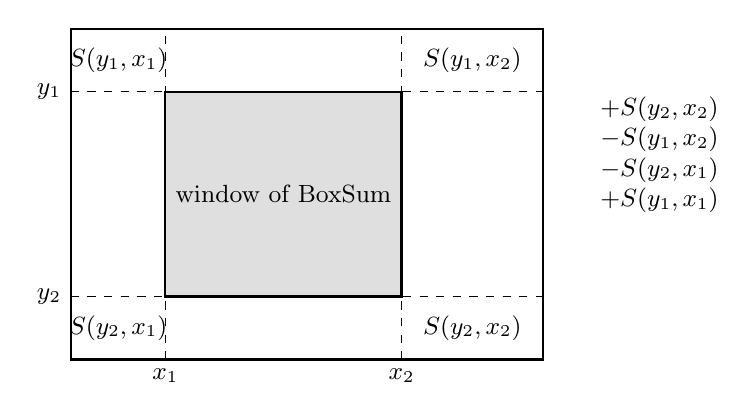
\begin{tikzpicture}[x=1cm,y=1cm]
\fill[gray!25] (1.2,0.8) rectangle (4.2,3.4);
\draw[thick] (0,0) rectangle (6,4.2);
\draw[thick] (1.2,0.8) rectangle (4.2,3.4);
\foreach \x/\l in {1.2/{$x_1$},4.2/{$x_2$}} {\draw[dashed] (\x,0) -- (\x,4.2); \node[font=\small,below] at (\x,0) {\l};}
\foreach \y/\l in {0.8/{$y_2$},3.4/{$y_1$}} {\draw[dashed] (0,\y) -- (6,\y); \node[font=\small,left] at (0,\y) {\l};}
\node[font=\small] at (2.7,2.1) {window of $\mathrm{BoxSum}$};
\node[font=\small] at (0.6,3.8) {$S(y_1,x_1)$};
\node[font=\small] at (5.1,3.8) {$S(y_1,x_2)$};
\node[font=\small] at (0.6,0.4) {$S(y_2,x_1)$};
\node[font=\small] at (5.1,0.4) {$S(y_2,x_2)$};
\node[font=\small,align=left,anchor=west] at (6.6,2.6) {$+S(y_2,x_2)$\\$-S(y_1,x_2)$\\$-S(y_2,x_1)$\\$+S(y_1,x_1)$};
\end{tikzpicture}
\caption{The four-corner rule of the summed-area table. Each table entry $S(y,x)$ is the sum of all pixels above and to the left of $(y,x)$ (measured with the vertical axis pointing down), so the shaded window sum follows from four entries (Equation~\ref{eq:seg-boxsum}).}
\label{fig:seg-boxsum}
\end{figure}

\paragraph{Dilation along one axis.}
The morphological dilation~\cite{haralick1987} that the block needs is always by a square, and a square dilation is separable into two one-dimensional dilations, each of which is again a window existence test and therefore again a cumulative sum.
With $c$ the cumulative sum of the boolean mask $m$ along the chosen axis, padded by $r+1$ before and $r$ after, the primitive is Equation~\ref{eq:seg-dilate},
\begin{equation}
\mathrm{AnyWithinRadius}(m,r)[i]=\bigl[\,c[i+2r+1]-c[i]>0\,\bigr]=\Bigl[\textstyle\bigvee_{k=-r}^{r} m[i+k]\Bigr],
\label{eq:seg-dilate}
\end{equation}
which is true wherever any set pixel lies within $r$ of position $i$ along that axis; applying Equation~\ref{eq:seg-dilate} once per axis dilates by a $(2r+1)\times(2r+1)$ square at a cost of two cumulative sums.
An \emph{erosion} of a mask is obtained as the dilation of its complement, complemented again, and a \emph{closing} as a dilation followed by an erosion; the block uses closings in three places and never needs any other structuring element.

\paragraph{Long straight runs along one axis.}
The second primitive answers, for every pixel, whether it lies on a run of at least $n$ consecutive set pixels along one axis.
With $c$ the cumulative sum of the mask along that axis, a run of length $n$ starts at index $i$ exactly when $c[i+n]-c[i]=n$; writing $\mathrm{hit}[i]$ for that indicator and $\mathrm{ch}$ for the cumulative sum of $\mathrm{hit}$, pixel $j$ is covered by some such run when Equation~\ref{eq:seg-runmask} holds,
\begin{equation}
\mathrm{LongRun}(m,n)[j]=\bigl[\,\mathrm{ch}[h_j+1]-\mathrm{ch}[l_j]>0\,\bigr],\qquad l_j=\max(0,j-n+1),\quad h_j=\min(j,L-n),
\label{eq:seg-runmask}
\end{equation}
where $L$ is the length of the axis and the window $[l_j,h_j]$ is the set of start positions of a run of length $n$ that could contain $j$; the mask is empty when $L<n$.
Equation~\ref{eq:seg-runmask} costs two cumulative sums and no loop, and it is the test on which the removal of printed rules in stage~4 rests.

\paragraph{The Gaussian kernel of the row profile.}
The only true Gaussian in the module is one-dimensional and short: the row-ink profile of stage~5 is smoothed by convolution with the 25-tap kernel of Equation~\ref{eq:seg-prof},
\begin{equation}
k[t]=\frac{\exp\bigl(-t^2/(2\sigma^2)\bigr)}{\sum_{u=-12}^{12}\exp\bigl(-u^2/(2\sigma^2)\bigr)},\qquad t=-12,\ldots,12,\qquad \sigma=4\ \text{rows},
\label{eq:seg-prof}
\end{equation}
so the kernel is truncated at exactly $3\sigma$, where the omitted tail carries about $0.3\,\%$ of the mass, and the normalisation makes the smoothed profile comparable with the raw one.
A standard deviation of four rows is about one tenth of a typical line pitch, which is enough to suppress the jitter caused by individual letters without merging two neighbouring line bodies into one peak.
Because the profile is a single vector of length $H$, a direct convolution costs $25H$ multiplications and no approximation is needed.

\paragraph{Equations retained from the earlier segmenter.}
An earlier segmenter approximated every blur as three successive box means of equal radius $r$~\cite{wells1986} \mustdo{confirm the page range of the Wells 1986 reference (IEEE TPAMI, vol.~8, no.~2) in the bibliography; it was left out rather than guessed.}, because the repeated convolution of a uniform kernel converges to a Gaussian shape by the central-limit argument.
A single box of full width $w=2r+1$ has the variance $(w^2-1)/12$, and three independent passes add their variances to
\begin{equation}
\sigma_{\mathrm{real}}^2=\frac{w^2-1}{4},\qquad w=2r+1,\qquad r=\max\Bigl(1,\;\mathrm{round}\Bigl(\tfrac12\sqrt{\tfrac{4\sigma^2}{3}+1}\Bigr)\Bigr),
\label{eq:seg-gauss}
\end{equation}
where $\sigma_{\mathrm{real}}$ is the realised standard deviation and $r$ the radius chosen for a requested nominal scale $\sigma$, so that $\sigma_{\mathrm{real}}\approx\sigma/\sqrt3\approx0.58\,\sigma$.
That earlier segmenter also converted a requested window width $B_w$ into an equivalent blur scale by the standard linear relation
\begin{equation}
\sigma_a=0.3\Bigl(\frac{B_w-1}{2}-1\Bigr)+0.8,
\label{eq:seg-sigmaa}
\end{equation}
in which $(B_w-1)/2$ is the window half-size.
\textbf{Neither Equation~\ref{eq:seg-gauss} nor Equation~\ref{eq:seg-sigmaa} is evaluated by the deployed module}, which uses a single box mean for the background (Equation~\ref{eq:seg-flat}) and the explicit kernel of Equation~\ref{eq:seg-prof} for the profile.
They are retained here, with their labels, because the segmentation timing figures reported in Section~\ref{sec:results} were measured on that earlier module and those figures include the cost of these constructions; a reader comparing the two must be able to see what was being timed.

\subsubsection{Stage 2: lighting normalisation and the ink mask}

The observed intensity of a photographed page is approximately paper reflectance times illumination, so the illumination is divided out rather than subtracted.
The background is estimated as a single box mean of the working grey image and the image is divided by it, Equation~\ref{eq:seg-flat},
\begin{equation}
\rho(p)=\frac{G(p)}{\max\bigl(\mathrm{BoxMean}_r(G)(p),\,1\bigr)},\qquad r=\max\Bigl(8,\;\min\bigl(40,\;\mathrm{round}(H/41)\bigr)\Bigr),
\label{eq:seg-flat}
\end{equation}
in which $G$ is the working grey image of stage~1, $H$ its height, $r$ the box radius, the clamp at 1 guards against division by a black background, and $\rho$ is the dimensionless \emph{ratio image} on which every threshold of the block acts.
On clean paper $\rho\approx1$ whatever the lighting; on ink $\rho$ is the local ink-to-paper reflectance ratio, which is a property of the pen and the paper and not of the lamp.
The radius of Equation~\ref{eq:seg-flat} is tied to the image height and clamped to $[8,40]$ so that it is always a few letter heights wide --- wide enough that a stroke does not darken its own background, narrow enough to follow a shadow edge --- and the clamp bounds the cost for a very large photograph.
Division rather than subtraction is used because the nuisance is multiplicative; subtracting a blurred copy would leave the ink contrast dependent on the local brightness, which is exactly what the next step must not depend on.
A limitation is that a large ink-heavy area, such as a dense diagram or a heavy correction block, is comparable in size with the blur window and therefore darkens its own background estimate, so its interior is partly flattened and may be lost.
Figure~\ref{fig:seg-illum} shows the effect on a real photograph.

\figplaceholder{5.2cm}{Four panels of the same photograph: (a) the colour photograph; (b) the working grey image $G$ after the $2{:}1$ box reduction; (c) the background estimate $\mathrm{BoxMean}_r(G)$ as a heat map, with the value of $r$ stated; (d) the ratio image $\rho$ of Equation~\ref{eq:seg-flat}. Source: call \texttt{SegmentLean.InkMask} on a personal page and save \texttt{BoxMean(gray,r)} and the returned \texttt{ratio} array; the module already returns $\rho$ as its second value, and the debug overlay it writes is $\rho$ scaled to 8 bits.}
\captionof{figure}{Lighting normalisation by division. The background estimate (c) follows the lighting gradient of the photograph, and dividing it out yields a ratio image (d) whose paper level is close to unity everywhere, on which a single global threshold is reliable.}
\label{fig:seg-illum}

\paragraph{A global threshold on the ratio image.}
Because the ratio image has already removed the slow shading, the ink decision can be a \emph{single global} threshold, which is chosen by Otsu's method~\cite{otsu1979}: the threshold that splits the histogram into a dark and a bright class so as to maximise the between-class variance, Equation~\ref{eq:seg-otsu},
\begin{equation}
t^*=\arg\max_t\;\omega_B(t)\,\omega_F(t)\,\bigl[\mu_B(t)-\mu_F(t)\bigr]^2,
\label{eq:seg-otsu}
\end{equation}
where $\omega_B(t)$ and $\omega_F(t)$ are the fractions of samples below and above $t$ and $\mu_B(t)$, $\mu_F(t)$ are the mean values of the two classes.
The product $\omega_B\omega_F$ is largest for a balanced split and the squared bracket largest for well-separated means, so Equation~\ref{eq:seg-otsu} places the cut where the two populations are most distinct.
The implementation evaluates the algebraically equivalent cumulative form of Equation~\ref{eq:seg-otsuimpl}, which needs one pass over the histogram and no inner loop,
\begin{equation}
\sigma_B^2(t)=\frac{\bigl[\mu_T\,\omega(t)-\mu(t)\bigr]^2}{\max\bigl(\omega(t)\,[1-\omega(t)],\;10^{-12}\bigr)},\qquad
\omega(t)=\sum_{i\le t}p_i,\quad \mu(t)=\sum_{i\le t} i\,p_i,\quad \mu_T=\mu(255),
\label{eq:seg-otsuimpl}
\end{equation}
in which $p_i$ is the normalised count of histogram bin $i$ and the clamp at $10^{-12}$ keeps the empty-class case finite.
The histogram has 256 bins spread uniformly over the ratio interval $[0,1.2]$, values outside being clipped into it, and the returned threshold is the centre of the winning bin, $t^*=(\arg\max+0.5)\times1.2/256$.
The upper limit 1.2 is deliberate: paper sits at $\rho\approx1$ and nothing above $1.2$ carries information about ink, so all of the resolution of the histogram is spent where the decision actually lies, and a specular highlight cannot drag the threshold.
The bin width is $1.2/256\approx0.0047$ in ratio units, which is far finer than the separation between ink and paper on any page tested.
A pixel is ink when $\rho<t^*$.

\paragraph{The solid-area veto.}
A global threshold on the ratio image still marks anything genuinely darker than its surroundings, which includes the interior of a binder shadow, a dark desk seen through a torn corner and the shaded gutter of a bound book.
Handwriting is thin: no pen stroke fills a $9\times9$ window completely.
The module therefore removes every region that does, Equation~\ref{eq:seg-solid},
\begin{equation}
\mathrm{solid}=\bigl[\mathrm{BoxMean}_4(\mathrm{ink})>0.999\bigr],\qquad
\mathrm{ink}\leftarrow\mathrm{ink}\wedge\neg\bigl[\mathrm{BoxMean}_3(\mathrm{solid})>0\bigr],
\label{eq:seg-solid}
\end{equation}
where $\mathrm{BoxMean}_4$ is the mean over a $9\times9$ window, so the first test is true only where all 81 pixels are ink, and the second test removes every pixel within a $7\times7$ window of such a centre, which strips the fringe of the blob as well as its interior.
The threshold 0.999 rather than 1 absorbs floating-point error in the integral image.
Equation~\ref{eq:seg-solid} is the one place where the block exploits a property of handwriting itself rather than of the photograph, and it is the reason the block tolerates a page photographed against a dark desk at all.
Its cost is that a very heavy marker stroke, or a filled-in letter counter in a large hand, is thinned at its centre; the halo recovery of stage~6 restores such pixels in the crop.

\paragraph{Why not a local threshold.}
A local adaptive threshold --- comparing each pixel with its own neighbourhood mean minus an offset --- is the usual answer for a photographed page, and it was what the earlier segmenter did, by Equation~\ref{eq:seg-adapt},
\begin{equation}
\mathrm{ink}(p)=\mathbb 1\bigl[\,I_{\mathrm c}(p)<M(p)-C\,\bigr]\wedge\mathrm{pageMask}(p),\qquad C=12,
\label{eq:seg-adapt}
\end{equation}
with $M$ a blurred copy of the corrected image, $\mathbb 1[\cdot]$ the indicator function and $C$ an offset in grey levels out of 255, together with a page-mask cut level derived from the median brightness $m_p$ inside the mask and $m_{bg}$ outside it,
\begin{equation}
c=\min\!\bigl(m_p-45,\;\max(m_p-85,\;\tfrac12(m_p+m_{bg}))\bigr).
\label{eq:seg-dark}
\end{equation}
\textbf{Neither Equation~\ref{eq:seg-adapt} nor Equation~\ref{eq:seg-dark} is evaluated by the deployed module}; both belonged to the earlier segmenter and are retained with their labels for the reason given above, namely that the timing figures of Section~\ref{sec:results} were measured on that module.
The deployed design replaces them with the single pair of Equations~\ref{eq:seg-flat} and~\ref{eq:seg-otsu} for three reasons that can be stated from the code alone.
First, the division has already removed the shading that the offset $C$ was there to survive, so the second local operation is redundant; second, a global threshold has no offset to tune, whereas $C$ in Equation~\ref{eq:seg-adapt} is a free parameter in grey levels that does not scale with pen contrast; and third, a local threshold necessarily marks \emph{something} in an empty region, because every region has a darkest pixel, which is precisely the behaviour that forced the earlier module's long chain of clean-up filters.
A threshold that also uses the local standard deviation~\cite{sauvola2000} would handle low-contrast regions better still, but it needs a second integral image of squared values and introduces two further constants; it was not adopted.
The cost of the global choice is honest and worth stating: a page whose illumination varies faster than the blur radius $r$ of Equation~\ref{eq:seg-flat} --- a hard shadow edge crossing the text, for instance --- is not corrected by the division, and a single global $t^*$ then either loses the dark side or floods the bright side.

\subsubsection{Stage 3: deskew by searching rotations}

If the text lines are tilted, a row-ink profile cannot resolve them, and the recogniser degrades as well.
The tilt is estimated by the classical projection-profile principle~\cite{postl1986}: when the lines are horizontal, the row-sum profile of the ink has sharp peaks at the line bodies and deep troughs between them, and any tilt smears both (Figure~\ref{fig:seg-skew}).
The module scores a candidate angle by the \emph{sum of squares} of the row profile, Equation~\ref{eq:seg-skew},
\begin{equation}
J(\theta)=\sum_y P_\theta(y)^2,\qquad P_\theta(y)=\sum_x R_\theta(y,x),\qquad \theta^*=\arg\max_\theta J(\theta),
\label{eq:seg-skew}
\end{equation}
where $R_\theta$ is the rotated ink mask and $P_\theta$ its row profile.
Equation~\ref{eq:seg-skew} is the variance criterion up to a constant: the total ink $\sum_y P_\theta(y)$ is very nearly invariant under rotation, so $\mathrm{Var}_y[P_\theta]=\frac1H\sum_yP_\theta^2-\bigl(\frac1H\sum_yP_\theta\bigr)^2$ differs from $J(\theta)/H$ by a term that is almost independent of $\theta$, and the two objectives have the same maximiser; the sum of squares is used because it needs no mean subtraction.
The search is a single exhaustive sweep of the 17 angles
\begin{equation*}
\theta\in\{-4.0^\circ,\,-3.5^\circ,\,\ldots,\,+3.5^\circ,\,+4.0^\circ\},
\end{equation*}
with no coarse-to-fine refinement, so the angular resolution is $0.5^\circ$ and the recoverable range is $\pm4^\circ$.
The mask that is rotated is the stage-2 ink mask reduced by a further factor two, that is one quarter of the photograph's linear size and one sixteenth of its area, so the whole search costs 17 rotations of a small mask plus 17 row sums.
Rotation about the image centre $(c_x,c_y)=((W-1)/2,(H-1)/2)$ uses inverse mapping,
\begin{equation}
\begin{pmatrix}x_s\\y_s\end{pmatrix}=\begin{pmatrix}\cos\theta&-\sin\theta\\ \sin\theta&\cos\theta\end{pmatrix}\begin{pmatrix}x-c_x\\y-c_y\end{pmatrix}+\begin{pmatrix}c_x\\c_y\end{pmatrix},
\label{eq:seg-rot}
\end{equation}
in which $(x,y)$ is an output pixel and $(x_s,y_s)$ the source position that is sampled.
Inverse mapping as in Equation~\ref{eq:seg-rot} is used, rather than mapping the source forward, because every output pixel then receives exactly one value and no holes can appear.
The candidate masks are rotated with nearest-neighbour sampling and a fill value of 0, so that the area outside the page contributes no ink and cannot flatten the profile; the page itself is then rotated once, bilinearly, with a fill value of 255, so that the corners brought in are white paper and not black.
Both the full-resolution page and the working image are rotated by the chosen $\theta^*$, and the ink mask and the ratio image are then \emph{recomputed} on the rotated working image, because the box mean of Equation~\ref{eq:seg-flat} is not rotation-equivariant.

\begin{figure}[h]
\centering
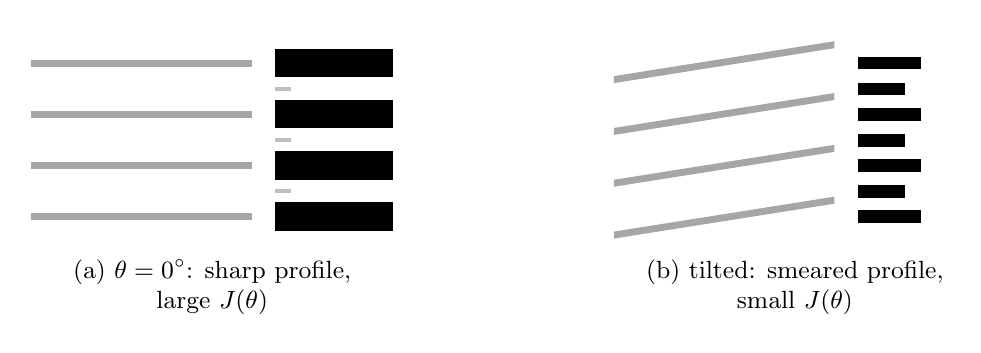
\begin{tikzpicture}[x=1cm,y=1cm]
% left: aligned lines
\begin{scope}
\foreach \k in {0,1,2,3} {\draw[line width=2.5pt,gray!70] (0,\k*0.65) -- (2.8,\k*0.65);}
\foreach \k in {0,1,2,3} {\fill[black] (3.1,\k*0.65-0.18) rectangle (3.1+1.5,\k*0.65+0.18);}
\foreach \k in {0,1,2} {\fill[black!25] (3.1,\k*0.65+0.3) rectangle (3.1+0.2,\k*0.65+0.35);}
\node[font=\small,align=center] at (2.3,-0.9) {(a) $\theta=0^\circ$: sharp profile,\\ large $J(\theta)$};
\end{scope}
% right: tilted lines
\begin{scope}[xshift=7.4cm]
\begin{scope}
\clip (0,-0.4) rectangle (2.8,2.4);
\foreach \k in {0,1,2,3} {\draw[line width=2.5pt,gray!70,rotate around={9:(1.4,1.0)}] (-0.4,\k*0.65) -- (3.2,\k*0.65);}
\end{scope}
\foreach \k in {0,1,2,3} {\fill[black] (3.1,\k*0.65-0.08) rectangle (3.1+0.8,\k*0.65+0.08);}
\foreach \k in {0,1,2} {\fill[black] (3.1,\k*0.65+0.24) rectangle (3.1+0.6,\k*0.65+0.40);}
\node[font=\small,align=center] at (2.3,-0.9) {(b) tilted: smeared profile,\\ small $J(\theta)$};
\end{scope}
\end{tikzpicture}
\caption{Principle of the projection objective of Equation~\ref{eq:seg-skew}. The bars on the right of each panel represent the row-sum profile of the ink. Aligned lines (a) give strong peaks and empty gaps and therefore a large sum of squares, whereas a tilt (b) fills the gaps and lowers it. The same profile is used again in stage~5 to find the line centres.}
\label{fig:seg-skew}
\end{figure}

\paragraph{Skew limitations and alternatives.}
The objective of Equation~\ref{eq:seg-skew} was preferred to a Hough transform~\cite{duda1972} of ink edges, because the latter is dominated by ruled lines and diagram strokes, whereas the projection objective is aligned with what the next stages need, namely a resolvable row profile; it is also the same quantity that stage~5 then reuses, so the page is scored by the criterion it is afterwards judged on.
Four limitations follow directly from the code and must be stated.
The range is only $\pm4^\circ$, so a page placed more crookedly than that is not straightened at all and the block will fail on it; the resolution is $0.5^\circ$, so a residual tilt of up to $0.25^\circ$ always remains, which over a 2000-pixel line is about 9 pixels of drift; a single global angle is estimated, so page curl and perspective keystone are not corrected; and the rotation is applied unconditionally, with no dead band around zero, so an already-straight page is resampled once for nothing, which costs a little sharpness.
The earlier segmenter searched $\pm8^\circ$ with a $0.1^\circ$ second pass and corrected the drift of each individual line afterwards by the least-squares fit of Equation~\ref{eq:seg-lsq} below; the deployed module does neither, and the residual per-line drift is simply carried into the crop.
One piece of design history belongs here: in the earlier module a sign mismatch between the rotation routine and the angle scorer was found to have \emph{doubled} the skew of every tilted page.
The deployed module is immune to that class of error by construction rather than by care, because the candidate masks are rotated by the same library call, with the same sign convention, that is afterwards applied to the page.
Figure~\ref{fig:seg-skewmeas} is reserved for a measured example of the objective.

\figplaceholder{4.4cm}{Skew search on a deliberately tilted photograph: left, a plot of $J(\theta)$ of Equation~\ref{eq:seg-skew} over the 17 candidate angles with the chosen $\theta^*$ marked; right, the page before and after rotation with the angle printed. Source: the loop inside \texttt{SegmentLines} that evaluates \texttt{max(np.arange(-4,4.01,0.5), key=...)}; store the score of every candidate instead of only the maximiser. The chosen angle is also returned in the statistics dictionary as the field \texttt{angle}.}
\captionof{figure}{Measured skew-search objective $J(\theta)$ (placeholder).}
\label{fig:seg-skewmeas}

\subsubsection{Stage 4: paper region, long straight runs and page-boundary artefacts}

A first estimate of the line pitch $P$ is now computed from the ink mask (the procedure is that of stage~5, applied here to the uncleaned mask) because every threshold of this stage is expressed in units of $P$.
Three removals then follow in order: everything outside the sheet, every long straight run, and every remaining piece of ink whose shape and position identify it as a page-boundary artefact rather than writing.

\paragraph{The paper region.}
The desk, a hand or a facing page must not contribute ink, so a boolean \emph{paper region} is estimated, and the construction exploits the fact that handwriting disappears under a sufficiently coarse average while the sheet does not.
The working grey image is reduced by a further factor $s=4$ by block averaging, blurred with a box mean of radius $\max(1,\lfloor0.15P/s\rfloor)$, and a cell is called dark when its value is below $0.45$ times the median of the reduced image.
If fewer than $0.2\,\%$ of the cells are dark there is no surround to cut away and the whole frame is accepted as paper, which is the correct answer for a photograph that is filled by the sheet.
Otherwise the bright set is labelled, its largest connected component is taken as the sheet, expanded back by a factor $s$ in each direction, and any rows or columns lost to the truncation of the reduction are counted as paper; the region is finally eroded by $\lfloor0.4P\rfloor$ on each axis with two applications of Equation~\ref{eq:seg-dilate}, so that the darkened rim of the sheet itself is not binarised as ink.
The factor $0.45$ on the median is the only brightness constant here, and it is a ratio rather than a level, so it survives a change of exposure; the erosion depth is in units of $P$, so it is about two fifths of a line spacing on any page.
The fraction of the frame that was accepted is reported as \texttt{paperCoverage} and the amount of ink discarded by this step as \texttt{inkOutsidePaper}, which makes the step auditable from the returned statistics alone.
The method fails when the desk is almost as bright as the paper, in which case the largest bright component swallows the desk; the fallback, as above, is the whole frame.
Figure~\ref{fig:seg-mask} is reserved for an example.

\figplaceholder{4.6cm}{Paper-region construction as a $2\times2$ panel: the $4\times4$-reduced blurred image, the dark set at $0.45\times$ its median, the largest bright component expanded back, and the final region after the $\lfloor0.4P\rfloor$ erosion overlaid on the photograph. Source: \texttt{SegmentLean.PaperRegionMask(g,P)}; the debug overlay that \texttt{SegmentLines} already writes (\texttt{\_cuts\_overlay.jpg}) tints everything outside this region red, so panel four can be cropped from it.}
\captionof{figure}{Construction of the paper region (placeholder).}
\label{fig:seg-mask}

\paragraph{Long straight runs: printed rules, underlines and the binder edge.}
Ruled paper, an underline and the straight shadow at the spine of a bound book all join words and lines into one giant piece of ink, and all three share one property that handwriting does not have: they are straight for longer than a line spacing.
The test is therefore the long-run primitive of Equation~\ref{eq:seg-runmask}, applied once per axis and bracketed by a dilation and a re-intersection so that a run broken by a slight tilt or by a crossing stroke still counts, Equation~\ref{eq:seg-cand},
\begin{equation}
\begin{aligned}
\mathrm{flat}&=\mathcal D_{1}^{y}\Bigl(\mathrm{LongRun}^{x}\bigl(\mathcal D_{1}^{y}(\mathrm{ink}),\;\lfloor1.25P\rfloor\bigr)\Bigr)\wedge\mathrm{ink},\\
\mathrm{upright}&=\mathcal D_{3}^{x}\Bigl(\mathrm{LongRun}^{y}\bigl(\mathcal D_{3}^{x}(\mathrm{ink}),\;\lfloor1.4P\rfloor\bigr)\Bigr)\wedge\mathrm{ink},
\end{aligned}
\label{eq:seg-cand}
\end{equation}
where $\mathcal D_r^{y}$ and $\mathcal D_r^{x}$ are the one-axis dilations of Equation~\ref{eq:seg-dilate} by radius $r$ along the row and the column axis, and the removed set is $\mathrm{flat}\vee\mathrm{upright}$.
The inner dilation is what makes Equation~\ref{eq:seg-cand} tolerant: dilating by one row before the horizontal run test lets a rule that drifts by a pixel over its length still read as a single run, and the generous radius of three columns for the vertical test absorbs the wobble of a photographed page edge.
The outer dilation grows the detected run back to the thickness it was given, and the final intersection with the ink mask guarantees that only pixels that were ink are removed.
The length thresholds are the essential point: a horizontal run must exceed $1.25P$ and a vertical run $1.4P$, both longer than any letter can be, since $P$ is the spacing between lines and a letter occupies well under half of it.
A long word written without a pen lift is not at risk, because a word is not straight to within one dilated row over $1.25P$.
The number of pixels removed is reported as \texttt{removedStraightPixels}.
The weakness of Equation~\ref{eq:seg-cand} is equally clear: a rule that is both faint and broken into fragments shorter than $1.25P$ survives it, and a deliberate long straight pen stroke --- a division bar in an equation, a strike-through --- is removed as though it were printed.
The earlier segmenter attacked the same problem by chaining short rule fragments across gaps, admitting a vertical offset of
\begin{equation}
|c_{y,b}-c_{y,a}|\le\Delta_{\max}=2\kappa+0.08\max(0,g)+0.04\,(w_a+w_b)
\label{eq:seg-slope}
\end{equation}
between two fragments separated by a gap $g$, where $c_y$ is a centroid row, $w$ a width and $\kappa$ a thickness cut.
\textbf{Equation~\ref{eq:seg-slope} is not evaluated by the deployed module}; it is retained with its label for the reason given above.
Dropping fragment chaining is a deliberate simplification --- it removed a group of constants ($\kappa$, the two slope allowances, the page-crossing span tests) at the cost of the broken-rule case just described.

\paragraph{Page-boundary artefact pieces.}
What survives the two steps above is still not all writing: edge slivers, corner shadows and fold creases remain, and they cannot be identified pixel by pixel because each is individually faint and locally indistinguishable from a stroke.
They are identified as whole \emph{pieces}.
The ink mask is closed by a square of radius $r_c=\max(1,\lfloor0.1P\rfloor)$ --- a dilation followed by an erosion, both by Equation~\ref{eq:seg-dilate} --- so that the pen lifts inside a word are bridged and a word becomes one piece, and the closed mask is labelled by the algorithm of the next subsubsection.
Every statistic is then accumulated over the \emph{original} ink pixels of each piece, so the closing decides what belongs together but never contributes area.
For a piece with area $A$, bounding box $[x_{\min},x_{\max}]\times[y_{\min},y_{\max}]$, height $h=y_{\max}-y_{\min}+1$ and width $w=x_{\max}-x_{\min}+1$, the module forms the predicates of Table~\ref{tab:seg-artifact} with $e=\max(3,\lfloor0.5P\rfloor)$ as the distance from the frame that counts as touching it.
Two of them need a measure of faintness, for which the mean ratio over the piece is compared with the page's own ink threshold, Equation~\ref{eq:seg-dark2},
\begin{equation}
\bar\rho_c=\frac{1}{A_c}\sum_{p\in c}\rho(p),\qquad \mathrm{faint}(c)=\bigl[\,\bar\rho_c>0.85\,t^*\,\bigr],
\label{eq:seg-dark2}
\end{equation}
where $t^*$ is the Otsu threshold of Equation~\ref{eq:seg-otsu} on the same ratio image.
A piece is faint when its average ink is only just past the threshold that admitted it; a real pen stroke is much darker than $0.85\,t^*$, whereas a crease or a printed rule sits barely below $t^*$ by construction, because that is how it got in.
Expressing faintness relative to $t^*$ rather than as a fixed level is what lets the same constant serve a pencil page and a fibre-tip page.
A further reference quantity is the \emph{text margin} $x_L$, the fifth percentile of the left edges of all letter-like pieces, a piece being letter-like when $A\ge0.065P^2$ and $h\le2.2P$; any piece lying entirely more than $1.2P$ to the left of $x_L$ is outside the text block and is discarded.
The number of pieces discarded is reported as \texttt{artifactPieces}.

\begin{table}[h]
\centering
\fontsize{9.5}{11.5}\selectfont
\begin{tabularx}{\linewidth}{|p{3.3cm}|X|}
\hline
\textbf{Discard condition} & \textbf{What it is meant to catch} \\
\hline
$x_{\min}\le e$ & Any piece touching the left frame edge: the sliver of the facing page or of the desk that the paper erosion left behind. \\
\hline
$x_{\max}\ge W-1-e$ and $w\le0.5P$ & A narrow sliver at the right frame edge; a real line reaching the right edge is wider than $0.5P$. \\
\hline
$y_{\min}\le e$ or $y_{\max}\ge H-1-e$, with $h\le0.5P$ and $w\le0.5P$ & A small fleck at the top or bottom frame edge. \\
\hline
$h>2.2P$ and $w\le0.5P$ & A tall thin streak spanning more than two line spacings: a binder edge or a fold. \\
\hline
$w\le0.12P$ and $h\ge1.2P$ & A vertical bar thinner than any letter and taller than any letter. \\
\hline
$\mathrm{faint}$, $w\le0.2P$ and $h\ge0.6P$ & A faint vertical bar: a printed margin rule or a crease. \\
\hline
$(y_{\min}\le e$ or $y_{\max}\ge H-1-e)$, $h\le1.2P$, $A/(hw)<0.15$, $\mathrm{faint}$ and $w>P$ & An edge shadow or fold: wide, faint, at an edge, and so sparse inside its own box that it cannot be writing. \\
\hline
$x_{\max}<x_L-1.2P$ & A piece entirely left of the text margin: a hole punch, a staple shadow, a page number in the gutter. \\
\hline
\end{tabularx}
\caption{The eight discard predicates applied to each closed piece of ink in stage~4, with $e=\max(3,\lfloor0.5P\rfloor)$, $x_L$ the fifth percentile of the left edges of letter-like pieces, and $\mathrm{faint}$ as defined by Equation~\ref{eq:seg-dark2}. The background label is exempt from all of them.}
\label{tab:seg-artifact}
\end{table}

The first row of Table~\ref{tab:seg-artifact} is the most aggressive rule in the module and its cost must be stated plainly: \emph{any} piece whose leftmost ink lies within $\max(3,\lfloor0.5P\rfloor)$ of the left edge of the frame is discarded regardless of its size or darkness, so a page photographed so tightly that the writing itself reaches the left edge loses the first letters of those lines.
The rule is safe for the intended use, in which the sheet is photographed with a visible margin, and it is the single rule that removes the facing page of an open book, which no shape test alone could do.
A second limitation of this stage is that it owns no model of what text \emph{is}: a diagram, a table or a stamp that is dark, compact and inside the text margin passes every predicate and is handed on to stage~5 as though it were writing.

\subsubsection{Stage 5a: connected components}

A \emph{connected component} is a maximal set of mask pixels that touch each other, diagonal neighbours included (8-connectivity).
Components are found with a run-length two-pass algorithm with union-find, a design that follows the classical sequential labelling idea~\cite{rosenfeld1966} but works on runs instead of single pixels.
Each image row is first encoded as maximal runs $[s,e)$ of set pixels, obtained from the differences of the row against a zero-padded copy of itself, so that a $+1$ marks a run start and a $-1$ a run end; no per-pixel loop is involved in finding the runs.
For every pair of adjacent rows the runs are swept with two pointers, and run $i$ of the upper row and run $j$ of the lower row are merged when they touch; for 8-connectivity the condition (Equation~\ref{eq:seg-adj}) is
\begin{equation}
s_i<e_j+1\ \ \wedge\ \ s_j<e_i+1,
\label{eq:seg-adj}
\end{equation}
and for 4-connectivity the $+1$ terms are dropped, where $s$ and $e$ are the start and end (exclusive) columns of the runs.
The pointer whose run ends first is advanced, so each row pair is swept once.
The merging uses a union-find structure with path halving~\cite{tarjan1984}, one of the one-pass compaction rules whose almost-linear amortised cost follows from Tarjan's analysis of path compression~\cite{tarjan1975}; the union itself always attaches the larger root index to the smaller, which keeps the labels of the first-seen components stable.
Roots are finally mapped to compact labels $1\ldots n$ by a sort-and-invert step, label 0 being the background, and the labels are painted back run by run.
The cost is linear in the number of runs times an almost constant factor, which is far cheaper than a pixel-wise method for thin handwriting strokes, where a run is typically several pixels long.
The routine is called on the closed mask (stage~4), on the raw mask (the dot rules of stage~6), inside the paper-region estimate, inside the pitch fallback and once per band when the fragment rule runs; it is the most frequently invoked primitive in the module.

\subsubsection{Stage 5b: line pitch and line centres from the row-ink profile}

This is the stage at which the deployed design departs most sharply from the earlier one, and the departure is in favour of the \emph{simpler} method, so the justification matters.

\paragraph{The profile.}
The row-ink profile is the number of mask pixels in each row, taken over the horizontal interval from $0.05W$ to $0.97W$ so that the extreme left and right of the frame cannot contribute, and smoothed with the Gaussian kernel of Equation~\ref{eq:seg-prof}:
\begin{equation}
\mathrm{prof}(y)=\sum_{x=\lfloor0.05W\rfloor}^{\lfloor0.97W\rfloor-1}\mathrm{ink}(y,x),\qquad \mathrm{sm}=\mathrm{prof}*k .
\label{eq:seg-pitch}
\end{equation}
A \emph{peak} of the smoothed profile is an interior row $y$ with
\begin{equation}
\mathrm{sm}(y)\ge\mathrm{sm}(y-1),\qquad \mathrm{sm}(y)>\mathrm{sm}(y+1),\qquad \mathrm{sm}(y)>0.06\max_u\mathrm{sm}(u),
\label{eq:seg-centres}
\end{equation}
the asymmetric pair of comparisons in Equation~\ref{eq:seg-centres} selecting the \emph{last} row of a flat plateau exactly once, so that a broad line body yields one peak and not a cluster of them, and the relative floor of $0.06$ of the maximum rejecting the ripple that stray marks leave between the lines.
The line pitch is then the median of the gaps between consecutive peaks,
\begin{equation*}
P=\mathrm{median}\bigl\{y_{i+1}-y_i\bigr\},
\end{equation*}
whenever at least two peaks exist, which is the case for every multi-line page.
Taking the median of the \emph{observed} gaps, rather than fitting one periodicity to the page, is what lets the pitch be right on a page whose paragraph spacing is irregular, and the module's own comment records that this choice was checked against sixteen real pages.

\paragraph{Three fallbacks.}
When fewer than two peaks are resolved, the pitch is estimated from the autocorrelation of the mean-removed smoothed profile $a=\mathrm{sm}-\overline{\mathrm{sm}}$: the non-negative-lag part of $a\star a$ is examined over lags $15$ to $\min(200,\lfloor L_{ac}/3\rfloor)$, and the first local maximum reaching $0.7$ of the segment maximum gives $P$.
The lower lag bound of 15 rows excludes the central spike and the upper bound of one third of the correlation length keeps the estimate inside the region where the correlation is still supported by enough overlap.
This branch is a fallback and not the primary method precisely because it can lock onto a \emph{multiple} of the true spacing on a page with uneven paragraph gaps, which the direct peak gap cannot.
If the autocorrelation gives nothing either --- a page with a single line of writing, where there is no spacing to measure --- the scale is taken from the letters themselves, by the median height of the plausible components, Equation~\ref{eq:seg-ht},
\begin{equation}
P=\max\bigl(15,\ \mathrm{round}\bigl(2.2\,\mathrm{median}\{h_c\}\bigr)\bigr),\qquad c:\ A_c\ge8\ \wedge\ 3\le h_c\le H,
\label{eq:seg-ht}
\end{equation}
where $h_c$ and $A_c$ are the height and the area of component $c$; the area floor of 8 pixels and the height floor of 3 rows exclude speckle, and the factor $2.2$ is the empirical ratio of line pitch to letter height for the hands in this project.
Equation~\ref{eq:seg-ht} is the only place where a glyph height still sets the scale, and it is a last resort rather than the primary unit, which is the substantive difference from the earlier segmenter: there, a median glyph height $\wht$ obtained by a median-of-medians over the components was the scale unit of the \emph{whole} block, so a page with one unusually large heading rescaled every threshold on it.
If no component qualifies at all, $P=48$ rows, an arbitrary but harmless default on a page that has no usable ink.

\paragraph{The line centres.}
The pitch and the profile are recomputed once on the \emph{cleaned} mask, after stage~4, because removing a ruled line or a shadow changes both.
The peaks of Equation~\ref{eq:seg-centres} are then turned into line centres by a greedy non-maximum suppression in units of the pitch: the peaks are visited in order of decreasing profile value and a peak is accepted as a centre only if it is at least $0.6P$ from every centre already accepted; the accepted set is finally sorted by row.
Visiting the strongest peak first means that where two peaks fall within $0.6P$ of each other --- the body of a line and the band of its own ascenders, for instance --- the one carrying more ink wins, which is the line body.
The separation floor of $0.6P$ is somewhat more than half a pitch, so two genuine lines can never be merged while a doubled peak inside one line can never be split.
Figure~\ref{fig:seg-chain} shows the profile, the centres and the seams of stage~6 together.

\paragraph{Why a row profile was chosen, and what it cannot do.}
The earlier segmenter rejected a row projection and grouped the components instead, by chaining each component to a successor on its right under the cost
\begin{equation}
\mathrm{cost}(a,b)=\max(0,\mathrm{gap})+3\,\Delta y,
\label{eq:seg-cost}
\end{equation}
with $\mathrm{gap}$ the horizontal distance between bounding boxes and $\Delta y$ the offset of the centroid rows, and by giving each resulting chain an area-weighted five-point moving-average baseline
\begin{equation}
\tilde y_i=\frac{\sum_{k=i-2}^{i+2}A_k\,y_k}{\sum_{k=i-2}^{i+2}A_k}.
\label{eq:seg-curve}
\end{equation}
\textbf{Neither Equation~\ref{eq:seg-cost} nor Equation~\ref{eq:seg-curve} is evaluated by the deployed module}, which uses the row profile of Equations~\ref{eq:seg-pitch} and~\ref{eq:seg-centres} instead; both are retained with their labels for the reason given above.
The reversal was deliberate and is justified as follows.
Chaining needs a correct component set before it can start, so every error of the clean-up stages propagates into the line structure, and it needs a chain-merging policy on top, which in the earlier module came to three passes with ten further constants and a quadratic worst case; the profile needs no component set at all, costs one pass over the mask, and produces the scale unit $P$ and the line centres from the same computation, so the page's own spacing calibrates the thresholds that are then applied to it.
Against that, three weaknesses of the profile are real and are accepted.
It assumes a single dominant horizontal orientation, so it is only as good as the $\pm4^\circ$ deskew that precedes it and it cannot represent a baseline that curves within one line; it assumes one column, so a two-column page or a diagram beside the text contributes peaks that belong to no single line and will be read as spurious lines or will corrupt $P$; and it has no notion of what text is, so it offers nothing like the text-versus-diagram separation the earlier module attempted.
A fourth weakness is a threshold rather than a principle: the floor of $0.06\max\mathrm{sm}$ in Equation~\ref{eq:seg-centres} will silently discard a line so faint or so short that its peak falls below six per cent of the strongest line's peak.
\mustdo{measure how often the $0.06\max\mathrm{sm}$ floor of Equation~\ref{eq:seg-centres} discards a real line. The quantity to report is the number of lines missed over the test pages, against the hand-counted line total; nothing in the project files records it.}
Finally, and most seriously, the module has no guard for the case in which \emph{no} peak clears that floor: an empty or near-empty page yields an empty set of centres, and the construction of the first cut then indexes the first centre of an empty list, which raises an exception rather than returning zero lines.
The same applies to the text margin $x_L$ of stage~4 when no piece is letter-like.
Both are blank-page failure modes, not misreadings, and the server should reject such an image before calling the block.

\subsubsection{Stage 6a: least-ink seams by dynamic programming}

The line centres say where the lines are; the boundaries between them are found as paths that cross as little ink as possible.
A straight horizontal cut halfway between two centres would sever every descender of the upper line and every ascender of the lower one, so the boundary is allowed to bend.
Between two consecutive centres $c_0<c_1$ the module builds the cost field of Equation~\ref{eq:seg-cost2} over the rows of that gap,
\begin{equation}
C(y,x)=4.0\,\tilde m(y,x)+0.012\left(\frac{y-\mu}{\max(1,(c_1-c_0)/2)}\right)^{\!2},\qquad \mu=c_0+\tfrac12(c_1-c_0),
\label{eq:seg-cost2}
\end{equation}
in which $\tilde m$ is the closed ink mask as a 0/1 field, $\mu$ the midline of the gap and the denominator a normalisation to the half-width of the gap, so that the second term is $0.012$ at the two centres and zero at the midline.
The first term of Equation~\ref{eq:seg-cost2} is the one that matters: with a weight of $4.0$ against a maximum of $0.012$ for the midline term, crossing a single ink pixel is more than three hundred times as expensive as sitting one half-gap away from the midline, so the path will take almost any detour to avoid ink and the midline term only breaks ties over the large empty areas between words.
Without that weak pull the path would wander arbitrarily far through the empty space and could leave the gap entirely; with it, the path traces real ink where there is ink and relaxes to a straight line where there is none.

The cheapest such path is found by dynamic programming over columns, Equation~\ref{eq:seg-seam},
\begin{equation}
A(y,x)=C(y,x)+\min_{|d|\le s}\bigl[\,A(y+d,\,x-1)+0.02\,|d|\,\bigr],\qquad s=7,
\label{eq:seg-seam}
\end{equation}
with $A(y,0)=C(y,0)$, where $d$ is the row displacement taken between column $x-1$ and column $x$ and the term $0.02|d|$ is a small penalty for not going straight ahead.
The chosen $d$ is stored for every cell, the path end is the row minimising $A(\cdot,W-1)$, and the path is recovered by following the stored displacements back to the first column.
Equation~\ref{eq:seg-seam} is exact: because the cost of a path is a sum over columns and the recursion considers every admissible predecessor, the value $A(y,x)$ is the true minimum cost of any admissible path from column 0 to cell $(y,x)$, and no search heuristic is involved.
The step limit $s=7$ rows per column is what lets the boundary react to a tall narrow descender rather than cutting through it, and the penalty $0.02$ per row of displacement --- weak against the ink weight $4.0$ but not negligible against the midline term --- keeps the path from zig-zagging where nothing forces it to move.
The mask used in Equation~\ref{eq:seg-cost2} is first closed by a square of radius $\max(2,\lfloor0.07P\rfloor)$; the module's own comment gives the reason, which is that a plain dilation would inflate every stroke into a blob and the cut would then trace the blob, whereas a closing fills only the thin gap beside a letter stem through which a path could otherwise thread, leaving the outer shape of the stroke close to the truth.
The outermost two boundaries are not computed but fixed: a constant row at $\max(0,c_{\mathrm{first}}-\lfloor0.75P\rfloor)$ above the first centre and at $\min(H-1,c_{\mathrm{last}}+\lfloor0.75P\rfloor)$ below the last, three quarters of a pitch being enough to contain the ascenders of the first line and the descenders of the last.
With $L$ centres there are therefore $L+1$ boundaries and $L$ bands.
Evaluating Equation~\ref{eq:seg-seam} costs $(2s+1)=15$ candidate comparisons per cell, and the cells of all gaps together are at most the rows of the page times its columns, so the whole seam computation is $O(15\,HW)$ in the worst case and in practice proportional to the ink-bearing height of the page.

\begin{figure}[h]
\centering
\begin{tikzpicture}[x=1cm,y=1cm]
% page area with three rows of text
\draw[thick] (0,0) rectangle (7.6,4.6);
% line 1 bodies
\foreach \x in {0.4,1.3,2.1,3.2,4.2,5.4,6.4} {\fill[gray!45] (\x,3.45) rectangle (\x+0.55,3.95);}
\fill[gray!45] (2.35,3.0) rectangle (2.5,3.5); % descender of line 1
% line 2 bodies
\foreach \x in {0.4,1.2,2.0,3.1,4.0,5.2,6.2} {\fill[gray!45] (\x,2.1) rectangle (\x+0.55,2.6);}
\fill[gray!45] (4.55,2.55) rectangle (4.7,3.15); % ascender of line 2
% line 3 bodies
\foreach \x in {0.4,1.4,2.4,3.4,4.5} {\fill[gray!45] (\x,0.75) rectangle (\x+0.55,1.25);}
% centres
\foreach \y/\l in {3.7/{$c_1$},2.35/{$c_2$},1.0/{$c_3$}} {
  \draw[dashed,gray] (0,\y) -- (7.6,\y);
  \node[font=\scriptsize,anchor=east] at (-0.08,\y) {\l};}
% seams
\draw[thick,red] plot[smooth,tension=0.7] coordinates {(0,3.05) (1.0,3.05) (2.0,3.05) (2.25,2.88) (2.6,2.88) (2.85,3.05) (4.0,3.05) (4.45,3.22) (4.8,3.22) (5.1,3.05) (6.4,3.05) (7.6,3.05)};
\draw[thick,blue] plot[smooth,tension=0.7] coordinates {(0,1.68) (1.5,1.68) (3.0,1.68) (4.5,1.68) (6.0,1.68) (7.6,1.68)};
% profile on the right
\begin{scope}[xshift=8.1cm]
\draw[->] (0,0) -- (0,4.6);
\draw[->] (0,0) -- (2.5,0) node[below,font=\scriptsize,anchor=north west] {$\mathrm{sm}(y)$};
\draw[thick] plot[smooth] coordinates {(0.05,0.2) (0.1,0.6) (0.9,1.0) (2.1,1.25) (0.9,1.45) (0.12,1.68) (0.08,1.9) (1.0,2.15) (2.3,2.35) (1.0,2.6) (0.1,2.85) (0.3,3.05) (0.12,3.25) (1.1,3.5) (2.25,3.7) (1.1,3.9) (0.1,4.15) (0.05,4.4)};
\draw[dashed,gray] (0,3.7) -- (2.4,3.7);
\draw[dashed,gray] (0,2.35) -- (2.4,2.35);
\draw[dashed,gray] (0,1.25) -- (2.4,1.25);
\fill[black] (2.25,3.7) circle (1.6pt);
\fill[black] (2.3,2.35) circle (1.6pt);
\fill[black] (2.1,1.25) circle (1.6pt);
\node[font=\scriptsize,anchor=west] at (2.4,3.7) {peak};
\draw[<->] (2.75,2.35) -- (2.75,3.7);
\node[font=\scriptsize,anchor=west] at (2.8,3.0) {$P$};
\end{scope}
\node[w2lab,anchor=south west] at (0.1,4.15) {seams bend around a descender and an ascender};
\end{tikzpicture}
\caption{Line pitch, centres and seams. The smoothed row-ink profile on the right has one peak per line body; the median gap between peaks is the pitch $P$ and the suppressed peaks are the line centres $c_i$ (Equations~\ref{eq:seg-pitch} and~\ref{eq:seg-centres}). Each boundary between two centres is the least-cost path of Equation~\ref{eq:seg-seam}, which detours around the descender of the line above and the ascender of the line below (red) and relaxes to a straight line where the gap is empty (blue).}
\label{fig:seg-chain}
\end{figure}

\subsubsection{Stage 6b: pixel ownership}

The seams divide the page into $L$ bands, and the default rule is the simplest possible one: an ink pixel belongs to the band it lies in.
Writing is not that tidy, however --- a descender crosses a seam, an $i$ dot sits a long way above its own line's body, a comma dangles below it --- so five correction rules act on top of the default, all of them stated in units of $P$ and $P^2$ and all of them conservative in the sense that a piece is only ever moved to an \emph{adjacent} band or dropped.
The band index of a pixel is obtained without any search, as the number of interior boundaries above it,
\begin{equation}
\mathrm{band}(y,x)=\sum_{n=1}^{L-1}\bigl[\,y\ge\mathrm{cut}_n(x)\,\bigr],
\label{eq:seg-band}
\end{equation}
Equation~\ref{eq:seg-band} is a single accumulation over the boundaries and gives $0$ for the top band and $L-1$ for the bottom one; pixels above the first boundary or below the last are outside every band and are never emitted.
For each piece $c$ of the closed labelling and each band $n$, the module counts the ink $N_{c,n}$ of that piece inside that band, and the ownership decision rests on the share
\begin{equation}
\mathrm{share}_{c,n}=\frac{N_{c,n}}{\sum_{m}N_{c,m}},\qquad
\mathrm{major}(c)=\begin{cases}\min\{n:\mathrm{share}_{c,n}\ge0.15\} & \text{if any share reaches }0.15,\\[2pt] \arg\max_n N_{c,n} & \text{otherwise.}\end{cases}
\label{eq:seg-share}
\end{equation}
A share of $0.15$ is the threshold at which a piece is held to have a genuine presence in a band, and the choice of the \emph{topmost} such band in Equation~\ref{eq:seg-share} rather than the largest is deliberate: when a piece really does span two lines, the crop that goes wrong if it loses the piece is the upper one, whose descender it is.
Figure~\ref{fig:seg-ramp} collects the size thresholds that the rules below use.

\begin{figure}[h]
\centering
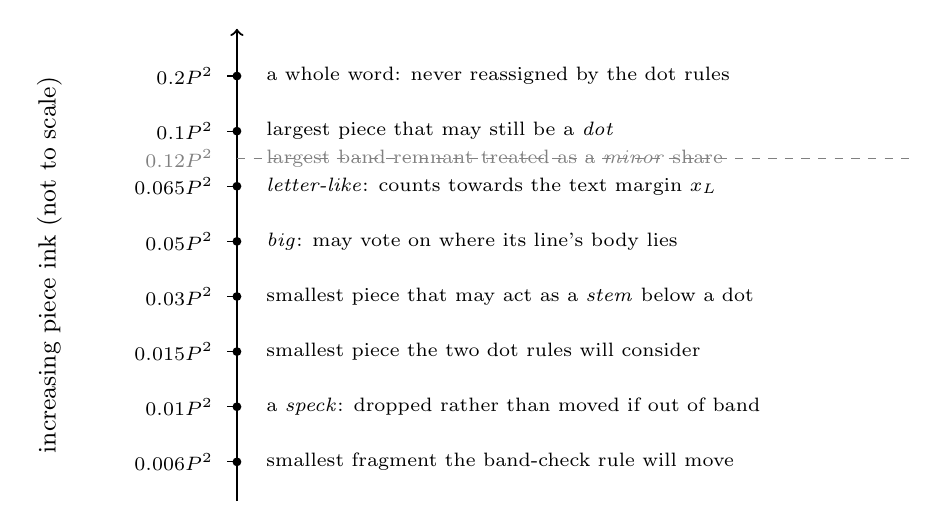
\begin{tikzpicture}[x=1cm,y=1cm]
\tikzset{sz/.style={font=\scriptsize,anchor=west}}
\draw[->,thick] (0,0) -- (0,6.0);
\node[font=\small,rotate=90,anchor=south] at (-2.1,3.0) {increasing piece ink (not to scale)};
\foreach \y/\v/\t in {
  0.5/{$0.006P^2$}/{smallest fragment the band-check rule will move},
  1.2/{$0.01P^2$}/{a \emph{speck}: dropped rather than moved if out of band},
  1.9/{$0.015P^2$}/{smallest piece the two dot rules will consider},
  2.6/{$0.03P^2$}/{smallest piece that may act as a \emph{stem} below a dot},
  3.3/{$0.05P^2$}/{\emph{big}: may vote on where its line's body lies},
  4.0/{$0.065P^2$}/{\emph{letter-like}: counts towards the text margin $x_L$},
  4.7/{$0.1P^2$}/{largest piece that may still be a \emph{dot}},
  5.4/{$0.2P^2$}/{a whole word: never reassigned by the dot rules}} {
  \fill[black] (0,\y) circle (1.6pt);
  \draw (0,\y) -- (-0.12,\y);
  \node[font=\scriptsize,anchor=east] at (-0.18,\y) {\v};
  \node[sz] at (0.25,\y) {\t};}
\draw[dashed,gray] (0,4.35) -- (8.6,4.35);
\node[font=\scriptsize,anchor=east,gray] at (-0.18,4.35) {$0.12P^2$};
\node[sz,gray] at (0.25,4.35) {largest band remnant treated as a \emph{minor} share};
\end{tikzpicture}
\caption{The piece-size ladder of stage~6b. Every size threshold in the ownership rules is a multiple of $P^2$, so the whole decision structure scales with the measured line pitch and none of it is tied to a pixel count. The entries are read from \texttt{SegmentLean.SegmentLines}.}
\label{fig:seg-ramp}
\end{figure}

\paragraph{Rule 1: minor remnants rejoin their own piece.}
A band in which a piece has a small, narrow remnant --- fewer than $0.12P^2$ pixels, less than $0.35$ of the piece's ink, in a band adjacent to its major one, and spanning at most $0.55P$ horizontally --- is not a line of its own but the tail of a letter that crossed the seam, and its pixels are given to the piece's major band.
The width condition is what separates the two cases that the ink count alone cannot: a cut-off tail is narrow, whereas a genuine short word in the next band is wide.

\paragraph{Rule 2: strays and specks.}
A piece with less than $0.06P^2$ of ink in total is too small to be a word.
Such a piece is first tested for company: the \emph{big} pieces (at least $0.05P^2$) that share its major band and lie within $6P$ horizontally are collected, and if there are none --- or if the piece is a \emph{speck} of under $0.01P^2$ and there are none even within $3P$ --- the piece is nowhere near any writing of that line and is dropped.
Otherwise the body of the line is located as the median centroid row of those neighbours (preferring those within $1.5P$ horizontally), and the piece is compared with it: if it sits more than $0.5P$ below that body it is moved down one band, and if more than $0.7P$ above it, up one band, a speck being dropped instead of moved in either case.
The asymmetry between $0.5P$ and $0.7P$ reflects the asymmetry of writing: a mark below the body of a line is usually a comma or a descender of that line, whereas a mark well above it is more often an accent belonging to the line above.
A second pass handles the intermediate sizes, between $0.06P^2$ and $0.15P^2$: such a piece simply joins whichever of its own band and the two neighbouring bands has its body closest in row to the piece's centroid.

\paragraph{Rule 3: a dot goes with the stem below it.}
An $i$ dot or a diaeresis floats above its line's body, often above the seam, and no size or position rule can place it correctly; what places it is the stem it belongs to.
A piece is a \emph{dot} when it is small and compact, Equation~\ref{eq:seg-dot},
\begin{equation}
A<0.1P^2,\qquad \max(h,w)\le0.45P,\qquad \max(h,w)\le2.2\max\bigl(\min(h,w),1\bigr),
\label{eq:seg-dot}
\end{equation}
the last condition of Equation~\ref{eq:seg-dot} bounding the aspect ratio at $2.2$ so that a short dash is not taken for a dot, and a \emph{stem} is any piece of at least $0.03P^2$ that is not a dot.
For each dot the module scans downwards up to $\lfloor0.4P\rfloor$ rows, over the columns of the dot widened by two on the left and three on the right, and takes the first stem it meets.
The dot is moved to that stem's band only if the geometry also agrees: the body of that band, measured as before over the big pieces within $1.5P$, must lie between $0.25P$ and $0.7P$ \emph{below} the dot, which is where an $i$ dot sits relative to its own x-height band.
The two conditions together are much stronger than either alone, because the vertical scan can meet the wrong stem on a crowded page and the band test can accept a mark that belongs to no stem.

\paragraph{Rule 4: a dot welded to the line above.}
The closing of stage~4 bridges gaps of up to $0.1P$, which occasionally welds an $i$ dot to a descender of the line above, so that the dot and that descender are one piece and rule~3 cannot see the dot at all.
This case is caught on the \emph{raw}, unclosed labelling, in which the dot is still separate.
A raw component qualifying as a dot by the test of Equation~\ref{eq:seg-dot} with the slightly wider bounds $0.015P^2\le A<0.1P^2$ and $\max(h,w)\le0.5P$ is followed downwards, as in rule~3, to the first raw stem; writing $n_1$ for the band that currently owns most of the dot's pixels and $n_2$ for the band of the stem, the dot's pixels are handed to $n_2$ only when all three of the following hold: $n_2=n_1+1$, so the move is downward by exactly one band; the closed piece containing the dot is smaller than $0.2P^2$, so that a whole word is never dragged across a seam; and the dot's own centre lies at least $0.45P$ below the centre of band $n_1$, so that a mark genuinely belonging to the upper line is not taken.

\paragraph{Rule 5: a ring at the foot of a stroke.}
The same welding produces a second, harder shape: the dot merges with the descender it touches and the pair reads as a stroke with a ring at its foot.
For each raw component the module takes the lowest ink pixel of each column, visits those columns in order of decreasing depth (at most sixty of them, with a horizontal exclusion of $\lfloor0.35P\rfloor$ around each one already visited so the same blob is not examined twice), and walks upwards from the lowest pixel while the component stays wide, stopping where the width falls below $0.45$ of the widest it has seen --- that is, where the blob narrows into the stem above it.
The shape is accepted as a welded dot only if its widest extent is between $0.2P$ and $0.45P$, its height-to-width ratio between $0.6$ and $1.6$, its height under $0.5P$, and --- the decisive test --- only if the blob \emph{encloses a hole}, which is checked by labelling the complement of the blob inside a one-pixel border and requiring more than one background component.
A dot ring encloses a hole; a hook or a loop tail at the end of a descender does not.
The reassignment then requires, exactly as in rule~4, that the band below be the next one, that the closed piece be under $0.2P^2$, and that the touch point lie no more than $0.45P$ above the centre of the receiving band.

\paragraph{Rule 6: a fragment with no ink in its own line's band.}
The rules above act on pieces; this last one acts on what the band assignment has actually produced.
For each band the pixels assigned to it are labelled afresh, and any resulting fragment of at least $0.006P^2$ that has \emph{no} pixel within $0.28P$ of that band's centre is, by definition, not part of that line's x-height body and is in the wrong place.
Such a fragment is first offered back to the line whose ink it touches: the fragment is dilated by two pixels, the bands of the mask pixels it then meets are counted, and if some other band is met at three or more pixels and that band is adjacent, and lies on the same side of the centre as the fragment does, the fragment moves there.
If the fragment touches nothing, the weaker positional test applies: it moves to whichever neighbouring band's centre is nearest, but only if that centre is within $0.2P$, that is only if the fragment genuinely lies in that line's x-height band.
Fragments placed by rules~4 and~5 are protected from this rule when they are small (under $0.04P^2$ and at most $0.4P$ across), because a dot deliberately lifted into a band has no ink near that band's centre and would otherwise be pushed straight back.
The conditions ``adjacent band'' and ``same side of the centre'' are what keep this rule from cascading: a fragment can move one band, in the direction its own position already indicates, and no further.

\subsubsection{Stage 6c: rendering the line crops}

The crops are rendered from the \emph{full-resolution}, lighting-normalised page, so the recogniser receives every pixel the camera captured even though all the decisions were taken at half resolution.
The background estimate computed at half resolution by Equation~\ref{eq:seg-flat} is enlarged to the full page by Equation~\ref{eq:seg-resize} and the full page is divided by it, which repeats the flat-field correction at full resolution without recomputing the integral image there.
The half-to-full scale factor is $f=W_{\mathrm{full}}/W$, and the bounding boxes reported to the caller are in full-resolution coordinates of the deskewed page.

A band is emitted as a line only if it carries enough ink and enough height: at least $\max(60,\,0.12\,\mathrm{median}_n N_n)$ owned pixels, where $N_n$ is the ink of band $n$, and a vertical extent of at least $\max(6,\,0.2P)$ rows.
The relative part of the ink floor is what makes this test work on a page of varying line lengths --- a short line is kept as long as it has an eighth of the typical line's ink --- and the absolute floor of 60 pixels catches the degenerate case of a page whose median is itself tiny.
The height floor is deliberately low, at a fifth of a pitch, because a line consisting only of short lower-case letters is a real line.
Within a band, a paragraph-sized vertical gap is then trimmed: the owned rows are split at empty rows into runs, the run carrying the most ink is kept, and the others are discarded --- but only if doing so removes more than $0.8P$ of height, so that the ordinary gap between a line's body and its own ascenders is never trimmed and only a stray mark a full line-spacing away is.

The bounding box of the surviving ink is padded by $\lfloor0.15P\rfloor$ on all four sides and scaled by $f$.
Inside that box the crop is composited from three layers.
The \emph{alpha} layer is the band's own ink mask, enlarged bilinearly, which gives a soft edge of one full-resolution pixel and avoids the staircase that nearest-neighbour enlargement would leave on every stroke.
The \emph{recovery} layer is the second tier of the two-tier ink description: a threshold computed afresh inside this crop, so that a pale line is judged against its own contrast and not the page's, by exactly the rule of Equations~\ref{eq:seg-flat} and~\ref{eq:seg-otsu} with the local radius $\max(3,\min(20,\mathrm{round}(h_{\mathrm{crop}}/8)))$.
That permissive mask is admitted only inside a halo of the band's own strong ink, obtained by dilating the band mask by $\max(1,\lfloor0.20P\rfloor)$ on each axis, and only where the ownership map does not already give the pixel to another band.
The composite is the double-threshold hysteresis rule of Canny's edge detector~\cite{canny1986}, applied to ink rather than to edge pixels, Equation~\ref{eq:seg-hyst},
\begin{equation}
\alpha=\max\Bigl(\alpha_{\mathrm{strong}},\ \ \mathbb 1[\rho_{\mathrm{local}}<t^*_{\mathrm{local}}]\cdot\alpha_{\mathrm{halo}}\cdot\mathbb 1[\text{not owned by another band}]\Bigr),
\label{eq:seg-hyst}
\end{equation}
in which $\alpha_{\mathrm{strong}}$ is the enlarged band mask, $\alpha_{\mathrm{halo}}$ the enlarged halo, $\rho_{\mathrm{local}}$ and $t^*_{\mathrm{local}}$ the ratio image and Otsu threshold of this crop alone, and the last factor is the ownership map enlarged by nearest-neighbour sampling.
The halo factor in Equation~\ref{eq:seg-hyst} is the strong-ink anchor that makes the recovery safe: a pale stroke is accepted when it is close to ink this line already owns, which bridges a letter the page-wide threshold missed, and it is refused when it stands alone, which is what would otherwise import the neighbouring line's ink or a smudge.
The ownership factor is an absolute veto, so recovery can never take a pixel that the page has already given to a neighbour, and the two crops of adjacent lines therefore cannot both claim the same ink.

The grey values are finally stretched so that the recogniser sees a consistent contrast whatever the pen, Equation~\ref{eq:seg-stretch},
\begin{equation}
\ell=\mathrm{clip}\!\left(\frac{255\,(v-b)}{\max(w-b,1)},0,255\right),\qquad
\mathrm{out}=255\Bigl(1-\bigl(\tfrac{255-\ell}{255}\bigr)^{0.55}\Bigr),
\label{eq:seg-stretch}
\end{equation}
where $v$ is the normalised grey value, $b$ is the 40th percentile of the values under the mask and $w$ the 75th percentile of the whole crop region.
Using the 40th percentile of the ink rather than its darkest pixel makes $b$ the \emph{typical} ink darkness, so a single very dark speck cannot flatten the whole line, and the 75th percentile of the region is a robust white point that a stray dark border cannot shift.
The exponent $0.55$ is below unity, which pulls the mid-tones towards black and therefore darkens a faint stroke much more than an already-dark one.
Outside the mask the crop is pure white, $255$, by the composite $\alpha\cdot\mathrm{out}+(1-\alpha)\cdot255$, so the recogniser never sees the paper texture or a neighbour's ink.
As a last step the crop is shifted horizontally so that its first column with $\alpha>0.1$ sits exactly $\lfloor \lfloor0.15P\rfloor f\rfloor$ pixels from the left edge, which gives every crop the same leading white margin; a constant left offset matters because the recogniser's input is left-flush (Equation~\ref{eq:seg-clf}) and a varying margin would shift the whole character sequence in time.

Each record returned holds the order index, the native-resolution crop, the $64\times640$ classifier canvas of Equation~\ref{eq:seg-clf} and the bounding box.
Alongside the records the module returns a debug overlay --- the ratio image in grey, the region outside the paper tinted red, and the boundaries drawn in alternating colours --- and a statistics dictionary with the fields \texttt{angle}, \texttt{pitch}, \texttt{paperCoverage}, \texttt{inkOutsidePaper}, \texttt{removedStraightPixels}, \texttt{artifactPieces}, \texttt{nLines} and \texttt{seconds}, which is how a page can be audited without instrumenting the module.
Figure~\ref{fig:seg-result} is reserved for an example output.

Two capabilities of the earlier segmenter are absent here and the absence is a design decision, not an oversight.
There is no text-versus-non-text tag: the earlier module scored every component for being a drawing, by
\begin{equation}
\begin{gathered}
\mathrm{holeScore}=\mathrm{clip}\!\Bigl(\frac{A_h/\wht^2-0.7}{0.8},0,1\Bigr),\qquad
\mathrm{sparse}=\begin{cases}0.7,&w>6\wht\wedge h>1.8\wht\wedge\mathrm{fill}<0.05\\0,&\text{otherwise}\end{cases}\\
\mathrm{mess}=\max(\mathrm{holeScore},\mathrm{sparse}),
\end{gathered}
\label{eq:seg-mess}
\end{equation}
with $A_h$ the area of the largest enclosed hole and $\wht$ the median glyph height, and emitted the high-scoring blocks as \texttt{MESS} items rather than text.
There is also no per-line deskew: the earlier module fitted a straight line $y=ax+b$ to the centroids of each line's components by area-weighted least squares,
\begin{equation}
\min_{a,b}\ \sum_i A_i\,(y_i-a\,x_i-b)^2,\qquad \phi=\arctan a,
\label{eq:seg-lsq}
\end{equation}
whose normal equations give the slope in closed form from the weighted sums of $x_i$, $y_i$, $x_i^2$ and $x_iy_i$ with no iteration, and rotated each crop by $-\phi$.
\textbf{Neither Equation~\ref{eq:seg-mess} nor Equation~\ref{eq:seg-lsq} is evaluated by the deployed module}; both are retained with their labels for the reason given above.
Dropping them has two consequences that Section~\ref{sec:results} must be read with: a diagram on a page is cut into line-shaped crops and passed to the recogniser, which will return nonsense for it, and the residual within-line baseline drift left by the $0.5^\circ$ skew resolution is carried into the crop instead of being corrected.
Both are accepted because the pages the system is used on are plain lined prose, and because the recogniser proved robust to a few degrees of residual drift; neither is defensible for a general document.

\figplaceholder{4.2cm}{Result of the block on a personal page: the debug overlay that the module already writes (\texttt{\_cuts\_overlay.jpg}, produced by running \texttt{python SegmentLean.py page.jpg outdir}), showing the ratio image with the paper region tinted and the seams of Equation~\ref{eq:seg-seam} drawn in alternating colours, next to three of the numbered crops from \texttt{outdir} and the corresponding $640\times64$ canvases from \texttt{outdir/classifier}.}
\captionof{figure}{Output of the segmentation block (placeholder).}
\label{fig:seg-result}

\subsubsection{Design history: the earlier segmenter}

The project had a first segmenter, \texttt{Software/CNN/SegmentPage.py}, whose entry point was \texttt{ProcessPage}.
It was a much larger program --- about 2200 lines and some sixty functions against the eleven of the deployed module --- and it worked in nine stages: it resized every photograph to a long side of 2400 pixels, built an explicit paper mask by a chain of ten morphological steps, applied a flat-field correction and then a local adaptive threshold with a fixed offset (Equations~\ref{eq:seg-adapt} and~\ref{eq:seg-dark}), excluded red ink by a colour test, removed printed structure in four separate passes including the fragment chaining of Equation~\ref{eq:seg-slope}, labelled the components and derived a median glyph height $\wht$ as the scale unit of the whole block (its own form of Equation~\ref{eq:seg-ht}), scored each component for being a diagram (Equation~\ref{eq:seg-mess}), grouped the components into lines by local chaining with a smoothed baseline (Equations~\ref{eq:seg-cost} and~\ref{eq:seg-curve}) followed by three chain-merging passes and a refinement step, and finally rendered the crops with a weak-ink hysteresis and the per-line deskew of Equation~\ref{eq:seg-lsq}.
It tagged its output \texttt{TEXT} or \texttt{MESS} and so could keep a diagram out of the recogniser.
That module is still in the repository and is still the module on which the segmentation timings of Section~\ref{sec:results} were measured, but \textbf{no part of the deployed pipeline calls it}: the server, the style-profile builder and the writer-classifier training program were all moved to \texttt{SegmentLean.SegmentLines}.

The move was made for three reasons.
First, the chain of clean-up filters existed mainly to repair the output of the local threshold, which marks something in every region; replacing that threshold with the division of Equation~\ref{eq:seg-flat} followed by one global Otsu cut on the ratio image removed the need for most of them, and with them a large number of constants that had each been tuned by hand on a few pages.
Second, grouping by chaining made the line structure depend on the component set, so any clean-up error propagated into it, and the chain-merging passes had a quadratic worst case and restarted after every merge; the row profile needs no component set, costs one pass, and yields the scale unit and the centres together.
Third, the glyph-height scale unit $\wht$ was fragile on a page with mixed writing sizes, whereas the line pitch $P$ is the quantity the segmentation problem is actually posed in.
What was given up is equally clear and has been stated above: text-versus-diagram tagging, per-line deskew, the broader $\pm8^\circ$ skew range with its $0.1^\circ$ resolution, and the chaining of broken rule fragments.

\subsubsection{Data sets, complexity, performance and limitations}

\paragraph{Use for the training data.}
The deployed module segments the photographed personal pages used for training as well as the pages submitted at inference time, because \texttt{BuildStyleProfile.py} and \texttt{TrainAuthor.py} call the same \texttt{SegmentLines} function as the server; there is therefore no train-to-deployment mismatch in the segmentation itself, which is the main practical argument for having only one segmenter.
The flat-scanned pages of the public database are not cut by this module at all: they are prepared by separate offline scripts under \texttt{Software/CNN/DatasetPrep}, which are not part of the deployed system.
The labels of those database pages were produced by reading the printed prompt of each form and aligning its word list with the detected ink word runs by dynamic programming, the global sequence alignment of Needleman and Wunsch~\cite{needleman1970} with a cost of the project's own choosing; the alignment cost for a run of measured width $a$ and an expected width $e$ is $c(a,e)=((a-e)/(e+1))^2$, with a penalty of 0.5 for the merging or splitting of words.

\paragraph{Complexity.}
Let $N_p=HW$ be the pixel count of the working image, which is one quarter of the photograph's.
Every thresholding, box-mean, dilation and long-run pass is $O(N_p)$ with a small constant, because each is one or two cumulative sums and four look-ups per pixel (Equations~\ref{eq:seg-boxsum}, \ref{eq:seg-dilate} and~\ref{eq:seg-runmask}); the number of such passes is fixed and does not grow with the page.
The skew search of Equation~\ref{eq:seg-skew} is 17 rotations and row sums of an image of $N_p/4$ pixels, so $O(17N_p/4)$.
Component labelling is linear in the number of runs times the almost-constant union-find factor~\cite{tarjan1975}, and it is invoked a fixed small number of times plus once per band in rule~6.
The dynamic program of Equation~\ref{eq:seg-seam} evaluates $2s+1=15$ candidates per cell over at most $N_p$ cells in total, so $O(15N_p)$, and it is the single most expensive array operation in the module.
The ownership rules are the only part not expressed as whole-array arithmetic: the two dot rules loop over the dot-shaped pieces, scanning at most $\lfloor0.4P\rfloor$ rows each, and the ring rule loops over the raw components, examining at most sixty columns each and walking at most $\lfloor0.5P\rfloor$ rows per column, so their cost is $O(n_{\mathrm{pieces}}\,P)$ and grows with the amount of writing rather than with the page area.
Peak memory is a handful of half-resolution arrays, one full-resolution normalised page, and one integral image per \texttt{BoxMean} call, each in double precision and of the same shape as its input.

\paragraph{Measured performance, and what was \emph{not} measured.}
This must be stated without hedging.
\textbf{The run time of the deployed segmenter was never measured.}
The segmentation timings quoted in Section~\ref{sec:results} --- the 24.8 to 69.1\,s per page, the share spent in component grouping, and the 25 to 32\,\% improvement from the two compiled replacements --- were all obtained from the \emph{earlier} module, \texttt{SegmentPage.ProcessPage}.
This is unambiguous from the stored measurement data: the timing field in \texttt{Report/FinalReport\_v3/qtp\_data/qtp4\_results.json} is literally named \texttt{stage1\_processpage\_s}, and the script that produced it imports \texttt{SegmentPage} and calls \texttt{ProcessPage}.
Those figures are therefore \emph{not} the cost of the block described in this section and must not be read as such.
No inference about the deployed module's speed is drawn from them here either: the deployed module is structurally much leaner --- it works on a quarter of the pixels, has no chain-merging passes and no nine-stage clean-up chain --- but ``leaner'' is not a measurement, and the one quantity that would settle it, the \texttt{seconds} field that \texttt{SegmentLines} itself returns on every call, was not collected into the results data.
\mustdo{measure the deployed segmenter. \texttt{SegmentLean.SegmentLines} already returns its own wall-clock time in the \texttt{seconds} field of its statistics dictionary; run it over the same pages and repeats on the development laptop, record the mean and the range, and repeat the run on the ODROID N2+. Until that is done, Section~\ref{sec:results} must continue to attribute its segmentation range explicitly to \texttt{SegmentPage.ProcessPage} and must state that the deployed module's own cost is unknown.}
\mustdo{the processing time of the block on the ODROID N2+ was not recorded in the project files; measure it.}
Whichever module is timed, the laptop figures that do exist are an order of magnitude above the 2\,s that requirement R4 allows for image capture and conditioning, so conditioning as implemented does not satisfy that budget; Section~\ref{sec:results} must report this, and must not claim the budget is met on the strength of the deployed module being leaner.
One further caution belongs here: Section~\ref{sec:discussion} proposes reducing the photograph before segmentation as a future saving, but the deployed module \emph{already} works at half resolution on each axis (stage~1), so that saving is in large part already taken and must not be counted twice.

\paragraph{Segmentation accuracy.}
A project note states that the earlier segmenter reproduced the hand-checked line count on a set of six pages; the test set and the scoring rule are not documented, so this statement is not used as evidence here, and in any case it was not obtained with the deployed module.
\mustdo{a quantified segmentation accuracy over the test pages for \texttt{SegmentLean.SegmentLines}, if it is claimed in Section~\ref{sec:results}. The simplest defensible measure is the detected line count against the hand-counted line count per page, reported per page and not only as a total, since a missed line and a spurious line cancel in a total.}

\paragraph{Design alternatives and justification.}
Table~\ref{tab:seg-alt} compares the main design choices of the deployed module with their alternatives; each chosen operation is the cheapest one robust against exactly one photographic nuisance.

\begin{table}[h]
\centering
\fontsize{9.5}{11.5}\selectfont
\begin{tabularx}{\linewidth}{|p{2.6cm}|X|X|}
\hline
\textbf{Decision} & \textbf{Alternative} & \textbf{Reason for the choice} \\
\hline
Lighting & Subtract a blurred background; no correction at all & The nuisance is multiplicative, so division (Equation~\ref{eq:seg-flat}) leaves an ink-to-paper ratio that does not depend on the lamp, whereas subtraction leaves the contrast brightness-dependent. \\
\hline
Ink threshold & Local mean minus an offset (Equation~\ref{eq:seg-adapt}, the earlier module); local mean and standard deviation~\cite{sauvola2000} & After the division the shading is already gone, so one global Otsu cut~\cite{otsu1979} on the ratio image suffices and has no offset to tune; a local rule necessarily marks something in an empty region, which is what forced the earlier module's long clean-up chain. \\
\hline
Blur & Direct Gaussian convolution; three box means (Equation~\ref{eq:seg-gauss}) & A single box mean over a summed-area table~\cite{crow1984} costs four look-ups per pixel at any radius, and the background estimate does not need a Gaussian profile. \\
\hline
Scale unit & Median glyph height $\wht$ (the earlier module); a fixed page size of 2400\,px & The line pitch $P$ is the quantity the problem is posed in, is measured on the page, and is unaffected by a heading of a different size; nothing then has to be resized to a fixed resolution. \\
\hline
Lines & Component chaining with a baseline curve (Equations~\ref{eq:seg-cost} and~\ref{eq:seg-curve}, the earlier module) & \emph{The deployed design uses the row-ink profile.} It needs no component set, so clean-up errors do not propagate into the line structure; it is one $O(N_p)$ pass instead of a quadratic merge; and it yields $P$ and the line centres from the same computation. Accepted cost: one column only, no curved baselines, no text-versus-diagram separation. \\
\hline
Line boundaries & A straight cut at the midline between centres & A straight cut severs every descender and ascender; the least-ink path of Equation~\ref{eq:seg-seam} bends around them, and the weak midline term keeps it straight where there is no ink to avoid. \\
\hline
Skew & Hough transform of edges~\cite{duda1972} & Edge directions are dominated by rules and diagram strokes; the projection objective~\cite{postl1986} is the same quantity the line-finding profile then uses. \\
\hline
Rule removal & Long morphological opening~\cite{haralick1987}; run-length chaining across gaps (Equation~\ref{eq:seg-slope}) & An opening erases long underlines and cross-bars and cannot follow a slope; the dilated long-run test of Equation~\ref{eq:seg-cand} tolerates slope and crossing strokes with two constants instead of five. \\
\hline
Faint filtering & A fixed darkness cut-off & Pen pressure and lighting differ per page; measuring faintness relative to the page's own Otsu threshold (Equation~\ref{eq:seg-dark2}) calibrates itself. \\
\hline
Text versus diagram & The hole-and-sparseness score of Equation~\ref{eq:seg-mess} (the earlier module); a learned layout detector & Not implemented in the deployed module. A learned detector is outside the first-principles scope; the score was dropped with the component-chaining stage it depended on, and the consequence --- a diagram is cut as if it were text --- is accepted for plain prose pages. \\
\hline
Per-line deskew & The area-weighted least-squares fit of Equation~\ref{eq:seg-lsq} (the earlier module) & Not implemented in the deployed module; the residual drift left by the $0.5^\circ$ skew resolution is carried into the crop, which the recogniser tolerates. \\
\hline
Page geometry & Four-point perspective warp & Not implemented; the camera looks straight down at the page, so keystone is small. \\
\hline
\end{tabularx}
\caption{Design alternatives of the deployed segmentation block. Rows that name an equation of the earlier segmenter record a capability that was deliberately given up.}
\label{tab:seg-alt}
\end{table}

\paragraph{Limitations.}
The block assumes left-to-right writing in a single column of roughly horizontal lines, and the following failures follow from the design rather than from tuning.
Skew beyond $\pm4^\circ$ is not corrected at all, and a residual of up to $0.25^\circ$ always remains and is not removed per line.
A page with two columns, or with a diagram beside the text, produces profile peaks that belong to no single line, so the line structure is wrong rather than merely imprecise; there is no text-versus-non-text tag, so a diagram is cut into line-shaped crops and read as nonsense.
A line whose profile peak is below six per cent of the strongest line's peak is silently lost, and a blank or near-blank page raises an exception instead of returning no lines, as does a page on which no piece of ink is letter-like.
Any piece of ink reaching within $\max(3,\lfloor0.5P\rfloor)$ of the left edge of the frame is discarded whatever its size, so the page must be photographed with a visible left margin.
A long deliberate pen stroke, such as a division bar or a strike-through, is removed as though it were a printed rule, while a faint rule broken into fragments shorter than $1.25P$ survives.
Illumination that varies faster than the background radius of Equation~\ref{eq:seg-flat} --- a hard shadow edge across the text --- is not corrected, and a single global threshold then loses one side of it.
A very heavy stroke that fills a $9\times9$ window is thinned by the solid-area veto of Equation~\ref{eq:seg-solid} and is only partly restored by the halo recovery.
Page curl and perspective are not corrected, and a desk nearly as bright as the paper defeats the paper region, whose fallback is the whole frame.
Finally, because the module is monochrome throughout, a coloured rule or a coloured correction is treated exactly like black ink and must be caught by the geometric tests alone.
